% ADDED figure (2026-11-02): the diagrams of one example box (C6a/C6b/§CA.7); generated by qft-C/tools/c6diag/figs/make_figs.sh
\tikzset{
  fdl/.style={line width=0.8pt, black},
  fdx/.style={circle, fill=black, inner sep=0pt, minimum size=3.6pt},
  fdv/.style={circle, fill=figB, draw=figB, inner sep=0pt, minimum size=5pt},
  fdlab/.style={font=\scriptsize, inner sep=2.6pt},
  fdmom/.style={->, >=Stealth, figO, line width=0.6pt},
}
\tikzset{
  fda/.style={fdl, postaction={decorate}, decoration={markings, mark=at position 0.55 with {\arrow{Stealth[length=5pt]}}}},
  fdS/.style={font=\small},
}
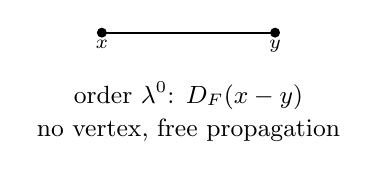
\begin{tikzpicture}[font=\small]
  \draw[fdl] (0,0)--(2.2,0); \node[fdx] at (0,0){}; \node[fdx] at (2.2,0){};
  \node[fdlab,below] at (0,0){$x$}; \node[fdlab,below] at (2.2,0){$y$};
  \node[fdS,align=center] at (1.1,-1.0) {order $\lambda^0$: $D_F(x-y)$\\[1pt] no vertex, free propagation};
\end{tikzpicture}
